Este capítulo possui como objetivo apresentar a plataforma de nuvens federadas BioNimbuZ, que foi selecionada para desenvolver o escalonador para plataformas heterogêneas proposto neste trabalho. A primeira sessão apresenta de forma geral o BioNimbuZ e descreve sua evolução ao longo do tempo. A segunda sessão descreve a arquitetura do BioNimbuZ, e suas principais partes, enquanto a última sessão foca sobre os escalonadores que existe atualmente no BioNimbuZ.

\section{Visão Geral}

O BioNimbuZ é uma plataforma livre de nuvens confederadas para execução de \textit{workflows} desenvolvida no \acrfull{LABID} por alunos de graduação e pós-graduação. Originalmente proposta por Saldanha\cite{Saldanha_BioNimbus} e refinada por alunos de iniciação científica, graduação, mestrado e doutorado\cite{closer12_BioNimbuZ_AHP}\cite{BioNimbuZ_6846526} \cite{6732620_BioNimbuZ_ACOsched}\cite{BioNimbuZ_Breno_Deric}\cite{BioNimbuZ_Vegara}\cite{BioNimbuZ_Willian_C99}.

É possível integrar nuvens de tipos de governança(vide capítulo 2), o que permite que cada provedor mantenha suas políticas e características internas, o que reduz a dependência da plataforma e, consequentemente, dos usuários de dependência de servidores específicos de nuvem. Essa funcionalidade é alcançada graças à facilidade e flexibilidade na inclusão de novos provedores na plataforma, através da utilização de \textit{plugins} de integração, que traduzem requisições vindas da plataforma para equivalentes específicas de cada servidor. O que é fundamental para evitar \textit{vendor lock-in}, que é a dependência de um serviço a um provedor em específico, por mais que existam outros.

Em sua concepção, a plataforma totalmente distribuída, utilizando comunicação \acrfull{P2P}, porém, durante sua evolução o BioNimbuZ se tornou centralizado em prol da simplicidade. Ainda assim, características que Saldanha propôs\cite{Saldanha_BioNimbus}, por exemplo tolerância a falhas, suporte a vários provedores de nuvens, elevado poder de armazenamento e processamento, foram não só mantidos, como também expandidos.

Moura \textit{el al.}\cite{BioNimbuZ_6846526} desenvolveram \acrfull{RPC}\cite{RPC_1701928} para a plataforma. Fazendo uso do Apache Avro\cite{Avro}, que possibilita comunicação de forma transparente entre computadores, para que seja possível a chamada de procedimentos em outros computadores via rede. Além disso, o núcleo do BioNimbuZ foi refatorado para utilização do serviço voltado para sistemas distribuídos Apache ZooKeeper\cite{Zookeeper}, e também foi implementado uma política de armazenamento que considera latência e o local em que o serviço seria executado, utilizando \acrfull{SFTP} para transferência de arquivos.

Barreiros\textit{el al.}\cite{BioNimbuZ_BioCirrus} refinaram a política de armazenamento, para que analisa-se a viabilidade de compactação de arquivos pré-transferência com base na largura de banda, tempo de transferência de arquivos e tempo de compressão e descompressão.

Ramos \textit{el al.}\cite{BioNimbuZ_Ramos} desenvolveu um controlador de \textit{jobs} para comunicação entre o núcleo do BioNimbuZ e a Camada de Interface com o Usuário, além de desenvolver uma interface gráfica que tornou a plataforma mais acessível.

Novamente, Barreiros\cite{BioNimbuZ_Willian_C99} desenvolveu o escalonador que se baseia no \textit{beam search} interativo multiobjetivo, chamado C99, com o objetivo de aumentar a eficiência do escalonamento, que passou a levar em consideração o custo por hora dos recursos a serem alocados.

Santos\cite{BioNimbuZ_Santos} refinou o serviço de armazenamento do BioNimbuZ, adicionando suporte ao uso de serviços de armazenamentos providos pelos diferentes provedores de nuvem, melhorando a praticidade e usabilidade da plataforma.

Ao longo dos trabalhos supracitados, que evoluíram o sistema proposto inicialmente por Saldanha\cite{Saldanha_BioNimbus}, o BioNimbuZ adquiriu uma arquitetura em camadas, que será descrita na próxima sessão.

\section{Arquitetura}
O BioNimbuZ foi implementado utilizando uma arquitetura de camadas, dispostas de forma hierarquizada e distribuída. Possui quatro camadas principais: Aplicação, Integração, Núcleo e Infraestrutura. Como expostos na figura \ref{Arquitetura}.

Internamente, o BioNimbuZ utiliza o Apache Zookeeper\cite{Zookeeper} para prover serviços de coordenação de ambientes distribuídos. Desenvolvido pela fundação Apache\cite{Apache}, tem como objetivo ser e fácil manuseio. Possui um modelo de dados semelhante a uma estrutura de diretórios
Uma outra tecnologia que também é utilizada no BioNimbuZ é o Apache Avro\cite{Avro}, para serialização de dados para transmissão pela rede.


\begin{figure}[htbp]
	%	\centerline{\includegraphics[scale=0.04]{img/EscalonadorProposto.png}}
	\centerline{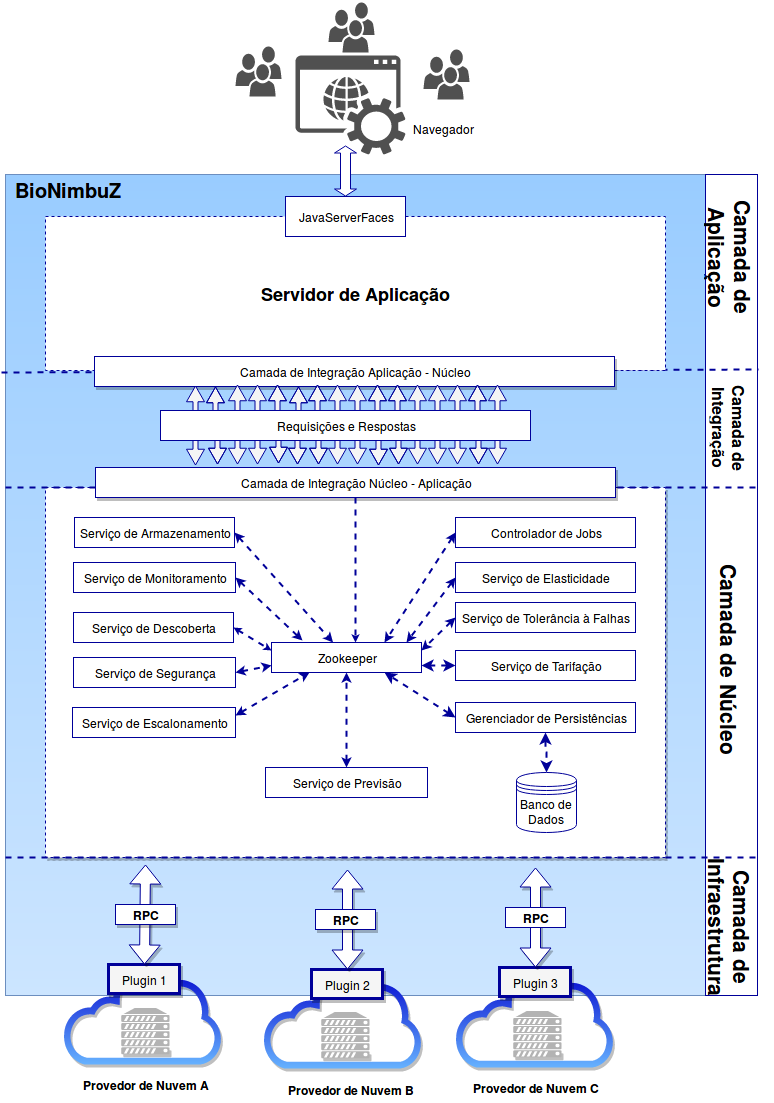
\includegraphics[scale=0.45]{img/ArquiteturaBioNimbuZ.png}}
	\caption{Arquitetura do BioNimbuZ}
	\label{Arquitetura}
\end{figure}



\subsection{Camada de Aplicação} Responsável por prover a interface de comunicação com o usuário, seja via uma interface gráfica(GUI), seja via \textit{web}. Após fazer login, o usuário pode enviar \textit{workflows} para serem executados e fazer \textit{upload} do arquivos necessários. Além de poder acompanhar o andamento de seus \textit{workflows} e pode obter, caso queira, o resultados parciais que já tiverem sido produzidos.

\subsection{Camada de Integração} Tem como objetivo de integrar as Camadas de Aplicação e de Núcleo, fazendo uso do \textit{framework} \acrshort{REST} para prover de forma prática essa funcionalidade, utilizando operações definidas no protocolo \textit{HTTP}, como \textit{GET}, \textit{DELETE} e \textit{PUT}.
Existem três tipos de mensagens trocadas entre o Núcleo e a camada de Aplicação:
\begin{itemize}
	\item \textit{Request}: Requisições da camada de Aplicação que contém todos os dados necessários para o seu processamento;
	\item \textit{Response}: Respostas que definem as mensagens enviadas da camada de Núcleo do BioNimbuZ; e
	\item \textit{Action}: Comandos a serem executados pelo núcleo, que são uma requisição enviada ao núcleo para se obter dados na resposta.
\end{itemize}
	
	\subsection{Camada de Núcleo} Realiza toda a gerência da federação, provendo vários serviços. Entre eles:

	\begin{itemize}
		\item Serviço de predição: Objetiva orientar o usuário do BioNimbuZ a escolher as melhores combinações de máquinas virtuais/provedores a partir da especificação do \textit{workflow} a ser executado e custo pretendido;
		\item Serviço de tarifação: Responsável por calcular o valor que os usuários devem pagar pelos serviços providndos do BioNimbuZ. Para tal, comunica-se com o serviço de monitoramento para obter informações como tempo de execução e quantidade de máquinas virtuais alocadas. É função desse serviço garantir o cumprimento das métricas de tarifação das nuvens integradas à federação, e repassar o valor ao usuário;
		\item Serviço de segurança: Realiza principalmente a autenticação de usuário, além de verificar as autorizações do mesmo. Contudo muitos outros aspectos de segurança computacional podem ser implementados por esse serviço, como criptografia na troca de mensagens;
		\item Serviço de Tolerância a Falhas: Como o nome diz, esse serviço é responsável em certificar que todos os serviços do BioNimbuZ estejam disponíveis o máximo de tempo possível. Além de ter a responsabilidade de tratar quaisquer falahas que venham a ocorrer. Tira vantagem da arquitetura distribuída do BioNimbuZ para prover redundância de dados;
		\item Serviço de Armazenamento: Posui a responsabilidade de gerenciar arquivos utilizados como entrada e/ou saída de cada estágio de um \textit{workflow}. Deve desempenhar seu papel de forma eficiente, do ponto de vista de custos de armazenamento e transmissão desses dados entre o local que está armazenado e o em que serão processados;
		\item Serviço de Escalonamento: Responsável por fazer o escalonamento de curto prazo de \textit{jobs}. Com curto prazo quer-se dizer que é tão somente o escalonamento de \textit{jobs} que estão prontas para serem executadas, à máquinas virtuais que os processarão. Não é responsabilidade do serviço de escalonamento lidar com dependências, pois essa responsabilidade é do controlador de \textit{jobs}.
%		No momento do início deste projeto, o BioNimbuZ possuia 5 políticas de escalonadonamento, são eles:
%		\begin{itemize}
%			\item AcoSched: Baseado em \textit{Load Balancing Ant Colony Scheduling}, desenvolvido por Oliveira. Baseado em heurística\cite{6732620_BioNimbuZ_ACOsched}
%			\item AHP: Baseado em \textit{Analytic Hierarchy Process}\cite{6732620_BioNimbuZ_ACOsched}
%			\item \textit{BasicSched}: Política \textit{First In First Out}, implementada no início da plataforma;
%			\item C99: Baseia-se no \textit{Beam Search} interativo multiobjetivo. \cite{BioNimbuZ_Willian_C99} Esse é o escalonador em uso atualmente.
%			\item \textit{RoundRobin}: O clássico escalonamento \textit{Round Robin};
%		\end{itemize}
	
	\end{itemize}
	
	\subsection{Camada de Infraestrutura} Disponibiliza uma interface de comunicação do BioNimbuZ com os provedores de nuvem. Utilizando \textit{plugins} para mapear requisições provenientes da Camada de Núcleo para comandos específicos de cada provedor.

O BioNimbuZ é capaz de ser integrado tanto à nuvens públicas quanto privadas, utilizando \textit{plugins} para permitir conexão com vários provedores de nuvem, cada qual com sua própria interface. Os \textit{plugins} não existem apenas na camada de integração: vários serviços da camada de núcleos também são disponibilizados como tal, provendo grande flexibilidade à plataforma.


\section{Serviço de Escalonamento}

Em suas primeiras fases de desenvolvimento, o escalonador do BioNimbuZ apenas realizava uma associação \acrfull{FIFO} ente as \textit{jobs} disponíveis e as \acrshort{VM}s disponíveis. Que rapidamente evoluiu para um escalonamento \textit{Round-Robin}. Desde então, fora propostas vários escalonadores a abordava várias metodologias diferentes, que serão explicados a seguir.

\subsection{\textit{Analytic Hierarchy Proccess}}
Em sua primeira versão oficial, o BioNimbuZ possuía um escalonador baseado no \acrfull{AHP}\cite{6732620_BioNimbuZ_ACOsched}, uma técnica de análise de decisões complexas, de amplo uso no meio corporativo. O problema é quebrado em uma estrutura hierárquica que cada elemento da herarquia interage apenas com níveis imediatamente superiores e inferiores. Após análise comparativa de como cada eleento interfere em todos os outros elementos dos níveis hierárquicos vizinhos, é obtido o resultado da análise, que revela as elhoreas opções com base nos critérios analisados.

\subsection{\textit{Ant Colony Optmization}}
Solução baseada na metaheurística \acrfull{ACO}\cite{ACO_DORIGO2005243} para o problemas de otimização combinatórias difíceis. Inspirado no comportamento de formigas enquanto andam. Oliveira \textit{el al.}\cite{6732620_BioNimbuZ_ACOsched} desenvolvera e iplementaram um escalonador para o BioNimbuZ com essa proposta de solução, que obteve resultados positivos comparados ao escalonador anterior, baseado no \acrshort{AHP}.

\subsection{\textit{Beam Search} Multiobjetivo}
O escalonador utilizado atualmente, desenvolvido por Barreiros\cite{BioNimbuZ_Willian_C99}, é um escalonador cuja proposta principal é ser interativo e multiobjetivo, ou seja, que pode ser interropido durante sua execução e ainda assim retornar um resultado válido, além de também levar em avaliar durante o processamento além da capacidade das máquinas virtuais disponíveis, o preço de cada uma delas. O escalonamento ocorre em três etapas:
\begin{enumerate}
	\item Busca gulosa para sobre conjuntos de Pareto para poda de conjuntos soluções localmente não ideias;
	\item \textit{Limited Discrepancy Search}, cujo objetivo é impedir que a poda conjuntos soluções que pode levar a u conjunto solução melhor futuramente; e
	\item \textit{Beam Search} Iterativo, que busca iterativamente os melhores conjuntos resultados.
\end{enumerate}

Uma funcionalidade que não foi abordada nos escalonadores citados acima é que eles não possuem suporte para rodar \textit{jobs} e \acrshort{GPU}s, esse é o objetivo deste trabalho. O próximo capítulo discorrerá sobre a implementação do escalonador proposto no capítulo anterior no BioNimbuZ.